\chapter{JFET en Saturación}
  \begin{wrapfigure}{R}{0.3\textwidth}
  \vspace{-1cm}
    \centering
    \resizebox{!}{\linewidth}{
    \begin{tikzpicture}
	\begin{pgfonlayer}{nodelayer}
		\node [style=none] (0) at (-2, 3.25) {};
		\node [style=none] (1) at (-2, -3.25) {};
		\node [style=none] (2) at (2, -3.25) {};
		\node [style=none] (3) at (2, 3.25) {};
		\node [style=none] (4) at (-2, 1.25) {};
		\node [style=none] (6) at (-1.25, 1.25) {};
		\node [style=none] (7) at (-1.25, -1.25) {};
		\node [style=none] (8) at (1.25, 1.25) {};
		\node [style=none] (9) at (1.25, -1.25) {};
		\node [style=none] (10) at (2, 1.25) {};
		\node [style=none] (11) at (2, -1.25) {};
		\node [style=none] (12) at (-2, -1.25) {};
		\node [style=none] (13) at (-2, 1.75) {};
		\node [style=none] (14) at (-0.75, 1.75) {};
		\node [style=none] (15) at (-0.75, -1.75) {};
		\node [style=none] (16) at (-2, -1.75) {};
		\node [style=none] (17) at (2, 1.75) {};
		\node [style=none] (18) at (0.75, 1.75) {};
		\node [style=none] (19) at (0.75, -1.75) {};
		\node [style=none] (20) at (2, -1.75) {};
		\node [style=none] (21) at (0, 0) {$n$};
		\node [style=none] (22) at (-1.5, 0) {$p$};
		\node [style=none] (23) at (1.5, 0) {$p$};
		\node [style=none] (24) at (-0.5, 3.25) {};
		\node [style=none] (25) at (-0.5, 3.5) {};
		\node [style=none] (26) at (0.5, 3.5) {};
		\node [style=none] (27) at (0.5, 3.25) {};
		\node [style=none] (28) at (-0.5, -3.25) {};
		\node [style=none] (29) at (-0.5, -3.5) {};
		\node [style=none] (30) at (0.5, -3.5) {};
		\node [style=none] (31) at (0.5, -3.25) {};
		\node [style=none] (32) at (-2, 0.5) {};
		\node [style=none] (35) at (-2.25, 0.5) {};
		\node [style=none] (36) at (2, 0.5) {};
		\node [style=none] (37) at (2, -0.5) {};
		\node [style=none] (38) at (2.25, -0.5) {};
		\node [style=none] (39) at (2.25, 0.5) {};
		\node [style=none] (40) at (-2.25, -0.5) {};
		\node [style=none] (41) at (-2, -0.5) {};
		\node [style=none] (42) at (-2.25, 0) {};
		\node [style=none] (43) at (-3.5, 0) {};
		\node [style=none] (44) at (2.25, 0) {};
		\node [style=none] (45) at (2.75, 0) {};
		\node [style=none] (46) at (2.75, 2.5) {};
		\node [style=none] (47) at (2, 2.5) {};
		\node [style=none] (48) at (-2, 2.5) {};
		\node [style=none] (49) at (-2.75, 2.5) {};
		\node [style=none] (50) at (0, 3.5) {};
		\node [style=none] (51) at (0, 4) {};
		\node [style=none] (52) at (0, -3.5) {};
		\node [style=none] (53) at (0, -4) {};
		\node [style=small dot] (54) at (-2.75, 0) {};
		\node [style=none] (55) at (0, 4.5) {D};
		\node [style=none] (56) at (0, -4.5) {S};
		\node [style=none] (57) at (-4, 0) {G};
	\end{pgfonlayer}
	\begin{pgfonlayer}{edgelayer}
		\draw [style=fill1] (3.center)
			 to [in=90, out=-90] (2.center)
			 to (1.center)
			 to (0.center)
			 to cycle;
		\draw [style=fill2] (7.center)
			 to (12.center)
			 to (4.center)
			 to (6.center)
			 to cycle;
		\draw [style=fill2] (8.center)
			 to (10.center)
			 to (11.center)
			 to (9.center)
			 to cycle;
		\draw [style=fill3] (6.center)
			 to (4.center)
			 to (13.center)
			 to (14.center)
			 to (15.center)
			 to (16.center)
			 to (12.center)
			 to (7.center)
			 to cycle;
		\draw [style=fill3] (8.center)
			 to (10.center)
			 to (17.center)
			 to (18.center)
			 to (19.center)
			 to (20.center)
			 to (11.center)
			 to (9.center)
			 to cycle;
		\draw [style=fill4] (32.center)
			 to (35.center)
			 to (40.center)
			 to (41.center)
			 to cycle;
		\draw [style=fill4] (39.center)
			 to (36.center)
			 to (37.center)
			 to (38.center)
			 to cycle;
		\draw [style=fill4] (25.center)
			 to (26.center)
			 to (27.center)
			 to (24.center)
			 to cycle;
		\draw [style=fill4] (29.center)
			 to (30.center)
			 to (31.center)
			 to (28.center)
			 to cycle;
		\draw (50.center) to (51.center);
		\draw (44.center) to (45.center);
		\draw (45.center) to (46.center);
		\draw (46.center) to (47.center);
		\draw (48.center) to (49.center);
		\draw (42.center) to (43.center);
		\draw (52.center) to (53.center);
		\draw (54) to (49.center);
		\draw [style=dashedd] (47.center) to (48.center);
	\end{pgfonlayer}
\end{tikzpicture}

    }
    \caption{estructura interna del JFET.}
    \label{fig:jfet.nopol}
  \end{wrapfigure}
  Si al JFET se le aplica un voltaje positivo $V_{DS}$ a través del canal y el gate está conectada directamente a la
  fuente, estableciendo la condición de $V_{GS} = 0 V$, el resultado es un gate y un source al mismo potencial y una
  región de empobrecimiento en el extremo bajo de cada material p similar a la distribución de las condiciones sin
  polarización, como se puede ver en la figura \ref{fig:jfet.nopol}. La región gris oscuro simboliza la región de
  empobrecimiento generada por la juntura de las regiones PN.

  En el instante en que se aplica $V_{DD} (= V_{DS})$, los electrones son atraídos hacia el drenaje y se establece la
  corriente convencional $I_D$. En este momento, el flujo de la carga está relativamente desinhibido y limitado sólo
  por la resistencia del canal n entre la fuente y el drenaje.

  \begin{wrapfigure}{l}{0.4\textwidth}
    \centering
    \resizebox{!}{\linewidth}{
    \begin{tikzpicture}
	\begin{pgfonlayer}{nodelayer}
		\node [style=none] (0) at (-2, 3.25) {};
		\node [style=none] (1) at (-2, -3.25) {};
		\node [style=none] (2) at (2, -3.25) {};
		\node [style=none] (3) at (2, 3.25) {};
		\node [style=none] (4) at (-2, 1.25) {};
		\node [style=none] (6) at (-1.25, 1.25) {};
		\node [style=none] (7) at (-1.25, -1.25) {};
		\node [style=none] (8) at (1.25, 1.25) {};
		\node [style=none] (9) at (1.25, -1.25) {};
		\node [style=none] (10) at (2, 1.25) {};
		\node [style=none] (11) at (2, -1.25) {};
		\node [style=none] (12) at (-2, -1.25) {};
		\node [style=none] (13) at (-2, 1.75) {};
		\node [style=none] (15) at (-1, -1.75) {};
		\node [style=none] (16) at (-2, -1.75) {};
		\node [style=none] (17) at (2, 1.75) {};
		\node [style=none] (19) at (1, -1.75) {};
		\node [style=none] (20) at (2, -1.75) {};
		\node [style=none] (21) at (0, 0) {$n$};
		\node [style=none] (22) at (-1.5, 0) {$p$};
		\node [style=none] (23) at (1.5, 0) {$p$};
		\node [style=none] (24) at (-0.5, 3.25) {};
		\node [style=none] (25) at (-0.5, 3.5) {};
		\node [style=none] (26) at (0.5, 3.5) {};
		\node [style=none] (27) at (0.5, 3.25) {};
		\node [style=none] (28) at (-0.5, -3.25) {};
		\node [style=none] (29) at (-0.5, -3.5) {};
		\node [style=none] (30) at (0.5, -3.5) {};
		\node [style=none] (31) at (0.5, -3.25) {};
		\node [style=none] (32) at (-2, 0.5) {};
		\node [style=none] (35) at (-2.25, 0.5) {};
		\node [style=none] (36) at (2, 0.5) {};
		\node [style=none] (37) at (2, -0.5) {};
		\node [style=none] (38) at (2.25, -0.5) {};
		\node [style=none] (39) at (2.25, 0.5) {};
		\node [style=none] (40) at (-2.25, -0.5) {};
		\node [style=none] (41) at (-2, -0.5) {};
		\node [style=none] (42) at (-2.25, 0) {};
		\node [style=none] (43) at (-3.5, 0) {};
		\node [style=none] (44) at (2.25, 0) {};
		\node [style=none] (45) at (2.75, 0) {};
		\node [style=none] (46) at (2.75, 2.5) {};
		\node [style=none] (47) at (2, 2.5) {};
		\node [style=none] (48) at (-2, 2.5) {};
		\node [style=none] (49) at (-2.75, 2.5) {};
		\node [style=none] (50) at (0, 3.5) {};
		\node [style=none] (51) at (0, 4) {};
		\node [style=none] (52) at (0, -3.5) {};
		\node [style=none] (53) at (0, -4) {};
		\node [style=small dot] (54) at (-2.75, 0) {};
		\node [style=none] (55) at (-0.5, 4.25) {D};
		\node [style=none] (56) at (-0.5, -4.25) {S};
		\node [style=none] (57) at (-4, 0) {G};
		\node [style=none] (59) at (-1, 2.25) {};
		\node [style=none] (61) at (-0.25, 1.75) {};
		\node [style=none] (62) at (0.25, 1.75) {};
		\node [style=none] (63) at (1, 2.25) {};
		\node [style=none] (64) at (-0.5, -2.75) {};
		\node [style=none] (65) at (-0.5, -1.75) {};
		\node [style=none] (68) at (0.25, -2) {};
		\node [style=none] (69) at (0.25, -1) {};
		\node [style=none] (70) at (-0.5, -1.25) {$e$};
		\node [style=none] (71) at (0.25, -0.5) {$e$};
		\node [style=none] (72) at (0, 0.75) {};
		\node [style=none] (73) at (0, 2.25) {};
		\node [style=none] (74) at (-0.5, 2.5) {};
		\node [style=none] (75) at (-0.5, 3) {};
		\node [style=none] (76) at (0.5, 2.5) {};
		\node [style=none] (77) at (0.5, 3) {};
		\node [style=none] (78) at (0, 4.5) {};
		\node [style=none] (79) at (4, 4.5) {};
		\node [style=none] (80) at (4, -4.5) {};
		\node [style=none] (82) at (-3.5, -4.5) {};
		\node [style=none] (83) at (0, -5.75) {};
		\node [style=none] (84) at (-0.5, -5.75) {};
		\node [style=none] (85) at (0.5, -5.75) {};
		\node [style=none] (86) at (0, -6.25) {};
		\node [style=none] (87) at (0, -6.75) {GND};
		\node [style=small dot] (88) at (0, -4.5) {};
		\node [style=none] (89) at (3.75, 0.25) {};
		\node [style=none] (90) at (4.25, 0.25) {};
		\node [style=none] (91) at (3.5, 0) {};
		\node [style=none] (92) at (4.5, 0) {};
		\node [style=none] (93) at (3.75, -0.25) {};
		\node [style=none] (94) at (4.25, -0.25) {};
		\node [style=none] (95) at (3.5, 0.5) {};
		\node [style=none] (96) at (4.5, 0.5) {};
		\node [style=none] (97) at (4, -0.25) {};
		\node [style=none] (98) at (4, 0.5) {};
		\node [style=none] (99) at (5, 0.25) {$V_{DD}$};
		\node [style=none] (100) at (3.25, 4) {$+$};
		\node [style=none] (101) at (3.25, -4) {$-$};
		\node [style=none] (102) at (-5, 0) {};
		\node [style=none] (103) at (-5, -4.5) {};
		\node [style=none] (104) at (-5, -2.75) {};
		\node [style=none] (105) at (-5, -1.75) {};
		\node [style=none] (106) at (-5, -2.25) {$V_{GS}=0V$};
		\node [style=none] (107) at (-2.5, -1.25) {};
		\node [style=small hollow dot] (108) at (0, 4) {};
		\node [style=small hollow dot] (109) at (0, -4) {};
		\node [style=small hollow dot] (110) at (-3.25, 0) {};
		\node [style=none] (111) at (0.75, 4.25) {};
		\node [style=none] (112) at (0.5, 4) {};
		\node [style=none] (113) at (1.5, 4.25) {};
		\node [style=none] (114) at (1.25, 3.75) {$I_D$};
		\node [style=none] (116) at (0.75, -4.25) {};
		\node [style=none] (117) at (1.5, -4.25) {};
		\node [style=none] (118) at (0.5, -4) {};
		\node [style=none] (119) at (1.25, -3.75) {$I_S$};
		\node [style=none] (120) at (3.25, 3.5) {};
		\node [style=none] (121) at (3.25, -3.5) {};
		\node [style=none] (122) at (3.25, -1) {};
		\node [style=none] (123) at (3.25, -2) {};
		\node [style=none] (124) at (3.25, -1.5) {$V_{DS}$};
		\node [style=none] (125) at (3.5, -0.5) {};
		\node [style=none] (126) at (4.5, 0.75) {};
	\end{pgfonlayer}
	\begin{pgfonlayer}{edgelayer}
		\draw [style=fill1] (3.center)
			 to [in=90, out=-90] (2.center)
			 to (1.center)
			 to (0.center)
			 to cycle;
		\draw [style=fill2] (7.center)
			 to (12.center)
			 to (4.center)
			 to (6.center)
			 to cycle;
		\draw [style=fill2] (8.center)
			 to (10.center)
			 to (11.center)
			 to (9.center)
			 to cycle;
		\draw [style=fill3] (61.center)
			 to [bend left=15, looseness=0.75] (15.center)
			 to (16.center)
			 to (12.center)
			 to (7.center)
			 to (6.center)
			 to (4.center)
			 to (13.center)
			 to (59.center)
			 to [bend left=60, looseness=1.50] cycle;
		\draw [style=fill3] (10.center)
			 to (17.center)
			 to (63.center)
			 to [bend right=60, looseness=1.50] (62.center)
			 to [bend right=15, looseness=0.75] (19.center)
			 to (20.center)
			 to (11.center)
			 to (9.center)
			 to (8.center)
			 to cycle;
		\draw [style=fill4] (32.center)
			 to (35.center)
			 to (40.center)
			 to (41.center)
			 to cycle;
		\draw [style=fill4] (39.center)
			 to (36.center)
			 to (37.center)
			 to (38.center)
			 to cycle;
		\draw [style=fill4] (25.center)
			 to (26.center)
			 to (27.center)
			 to (24.center)
			 to cycle;
		\draw [style=fill4] (29.center)
			 to (30.center)
			 to (31.center)
			 to (28.center)
			 to cycle;
		\draw (50.center) to (51.center);
		\draw (44.center) to (45.center);
		\draw (45.center) to (46.center);
		\draw (46.center) to (47.center);
		\draw (48.center) to (49.center);
		\draw (42.center) to (43.center);
		\draw (52.center) to (53.center);
		\draw (54) to (49.center);
		\draw [style=dashedd] (47.center) to (48.center);
		\draw [style=arrow] (64.center) to (65.center);
		\draw [style=arrow] (68.center) to (69.center);
		\draw [style=arrow] (74.center) to (75.center);
		\draw [style=arrow] (76.center) to (77.center);
		\draw [style=arrow] (72.center) to (73.center);
		\draw (79.center) to (78.center);
		\draw (78.center) to (51.center);
		\draw (43.center) to (82.center);
		\draw [style=fill4] (85.center)
			 to (83.center)
			 to (84.center)
			 to (86.center)
			 to cycle;
		\draw [style=fill4] (82.center) to (88);
		\draw [style=fill4] (53.center) to (88);
		\draw [style=fill4] (80.center) to (88);
		\draw [style=fill4] (88) to (83.center);
		\draw (95.center) to (96.center);
		\draw (89.center) to (90.center);
		\draw (91.center) to (92.center);
		\draw (93.center) to (94.center);
		\draw (98.center) to (79.center);
		\draw (97.center) to (80.center);
		\draw [style=end] (105.center) to (102.center);
		\draw [style=end] (104.center) to (103.center);
		\draw (113.center) to (111.center);
		\draw [style=arrow, bend left=315] (111.center) to (112.center);
		\draw [style=arrow] (116.center) to (117.center);
		\draw [bend right=45] (118.center) to (116.center);
		\draw (120.center) to (122.center);
		\draw (123.center) to (121.center);
		\draw [style=arrow] (125.center) to (126.center);
	\end{pgfonlayer}
\end{tikzpicture}

    }
    \caption{JFET polarizado.}
    \label{fig:jfet.pol-sat}
  \end{wrapfigure}
  Conforme el voltaje $V_{DS}$ aumente de $0V$ a algunos volts, la corriente también lo hará de acuerdo con la ley de Ohm.
  Al mismo tiempo, las regiones de empobrecimiento se iran acercando mas y mas, hasta llegar a un potencial $V_p$, en el
  cual las regiones se tocan y se produce un estrangulamiento. La palabra estrangulamiento puede llegar a interpretarse
  como que "deja de circular corriente", pero en realidad sigue existiendo un canal muy pequeño, con una corriente de
  muy alta densidad.

  A medida que $v_{DS}$ aumenta más allá de $V_p$ , la longitud de la región del encuentro cerca no entre las dos
  regiones de empobrecimiento crece a lo largo del canal, pero el nivel de $I_D$ permanece igual. Por consiguiente, una
  vez que $V_{DS} > V_p$, el JFET tiene las características de una fuente de corriente. Como se muestra en la figura
  6.9, la corriente se mantiene fija en el valor $I_D = I_{DSS}$ , pero la carga aplicada determina el voltaje $V_{DS}$
  (para niveles $\geq V_p$).

  \section{Actividad de Simulación}
    Se propuso implementar el circuito de la figura \ref{crkt:jfet-sat} en el simulador LTSpice, y hacer que la fuente
    $V1$ varíe desde $0V$ a $15V$ en pasos de $0.1V$, para poder recrear una curva que exponga el comportamiento de la
    corriente $I_D$ en función del voltaje drain-source $V_{DS}$.
    \begin{figure}[!ht]
      \centering
      \begin{minipage}{0.45\textwidth}
        \begin{tikzpicture}
          % Paths, nodes and wires:
          \node[njfet](N1) at (0, -0){} node[anchor=west] at (N1.text){$BF245B$};
          \draw (2.5, 0.75) to[battery, l={$V1$}] (2.5, -0.75);
          \draw (2.5, 0.73) -- (2.5, 2.48) |- (0, 2.48) -| (0, 0.75);
          \draw (0, -0.77) -- (0, -2);
          \draw (2.5, -0.75) -- (2.5, -2);
          \draw (-0.98, -0.27) -| (-2, -2);
          \node[ground] at (-2, -2){};
          \node[ground] at (0, -2){};
          \node[ground] at (2.5, -2){};
        \end{tikzpicture}
        \caption{circuito de prueba para saturación.}
        \label{crkt:jfet-sat}
      \end{minipage}
      \hfill
      \begin{minipage}{0.45\textwidth}
        \begin{lstlisting}[style=ltspice, caption={Parámetros de simulación LTspice}, label=list:jfet-sat]
.MODEL  BF245B   NJF VTO = -2.3085E+000 BETA = 1.09045E-003 LAMBDA = 2.31754E-003 RD = 7.77648E+000 RS = 7.77648E+000 IS = 2.59121E-016 CGS  = 2.00000E-012 CGD  = 2.20000E-012 PB = 9.91494E-001 FC = 5.00000E-001
.dc V1 0 15 .1
        \end{lstlisting}
      \end{minipage}
    \end{figure}

    \begin{figure}[!ht]
      \centering
      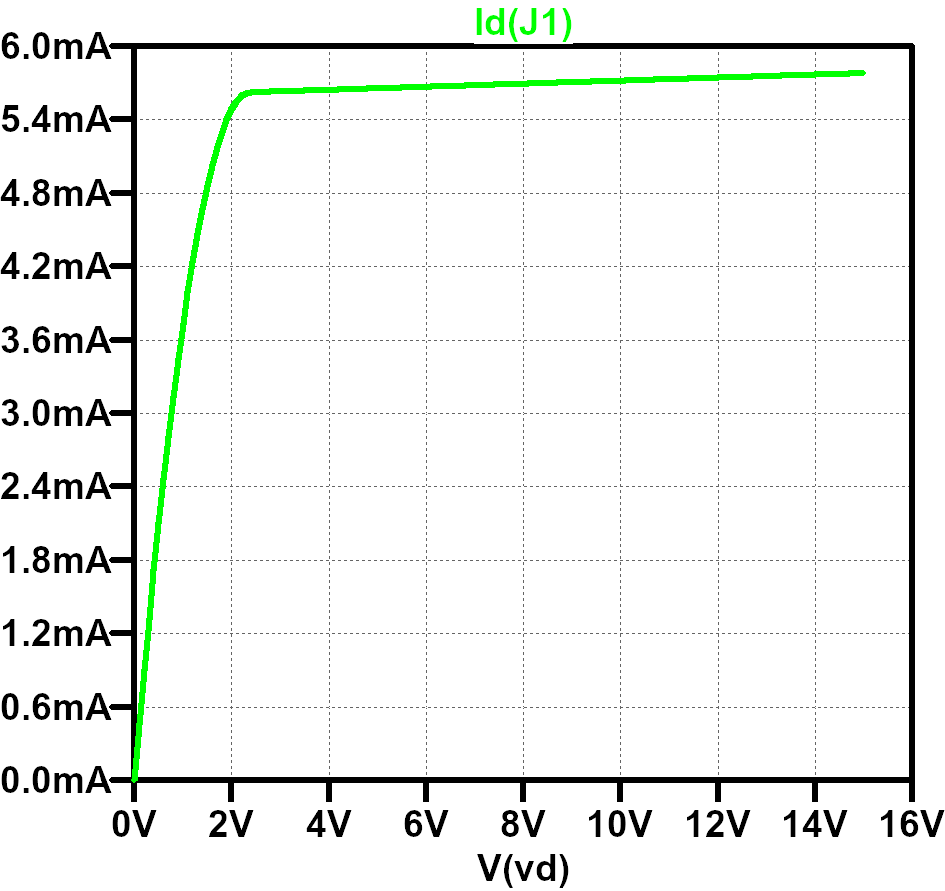
\includegraphics[width=0.8\textwidth]{images/saturacion-id_vds.png}
      \caption{resultados de simulación para saturación del JFET.}
      \label{fig:sim.sat}
    \end{figure}
    En la figura \ref{fig:sim.sat} puede observar los resultados de la simulación. Como se puede ver, a partir de
    aproximadamente $2V$, el JFET llega a su corriente $I_{DSS}$. A pesar de que el voltaje $V_{DS}$ sigue aumentando, la
    corriente $I_D$ permanece prácticamente constante.

    La hoja de datos especifica una $I_{DSS}$ que va de $6mA$ a $15mA$. El modelo que se utilizo usa el mínimo de
    corriente $I_{DSS}$, lo cual se corrobora en la gráfica de la figura \ref{fig:sim.sat}, estabilizándose al rededor
    de los $5.5mA$.

  \section{Actividad de Laboratorio}
